%%%%%%%%%%%%%%%%%%%%%%%%%%%%%%%%%%%%%%%%%%%%%%%%%%%%%%%%%%%%%%%
%
% Optimized LaTeX Diagram Code
%
%%%%%%%%%%%%%%%%%%%%%%%%%%%%%%%%%%%%%%%%%%%%%%%%%%%%%%%%%%%%%%%
\documentclass[border=5pt]{standalone}
\usepackage{tikz}
\usepackage{amsfonts,amsmath,amssymb,amsthm}
\usetikzlibrary{shapes.geometric, arrows}
\newcommand{\dd}{\text{\normalfont d}}
\newcommand{\dt}{\text{\normalfont d}t}
\newcommand{\ds}{\text{\normalfont d}s}
\newcommand{\du}{\text{\normalfont d}u}
\newcommand{\dr}{\text{\normalfont d}r}
\newcommand{\dx}{\text{\normalfont d}x}
\newcommand{\dX}{\text{\normalfont d}X}
% \tikzstyle{startstop} = [circle, 
% minimum width=1.2cm, 
% minimum height=1.2cm,
% text centered, 
% draw=black, 
% fill=gray!20]

% \tikzstyle{unit} = [rectangle, 
% minimum width=1.2cm, 
% minimum height=1.2cm, 
% text centered, 
% text width=1.5cm, 
% draw=black, 
% fill=orange!30]

% \tikzstyle{box} = [rectangle, 
% minimum width=2.2cm, 
% minimum height=2.2cm, 
% text centered, 
% draw=black, 
% fill=green!30]

\tikzstyle{box} = [rectangle, 
minimum width=13.2cm, 
minimum height=1.2cm, 
text centered, 
draw=black, 
fill=green!30]

\tikzstyle{nonactivebox} = [rectangle, 
minimum width=13.2cm, 
minimum height=1.2cm, 
text centered, 
draw=black, 
fill=gray!30]

\tikzstyle{arrow} = [thick,->,>=stealth]

\begin{document}

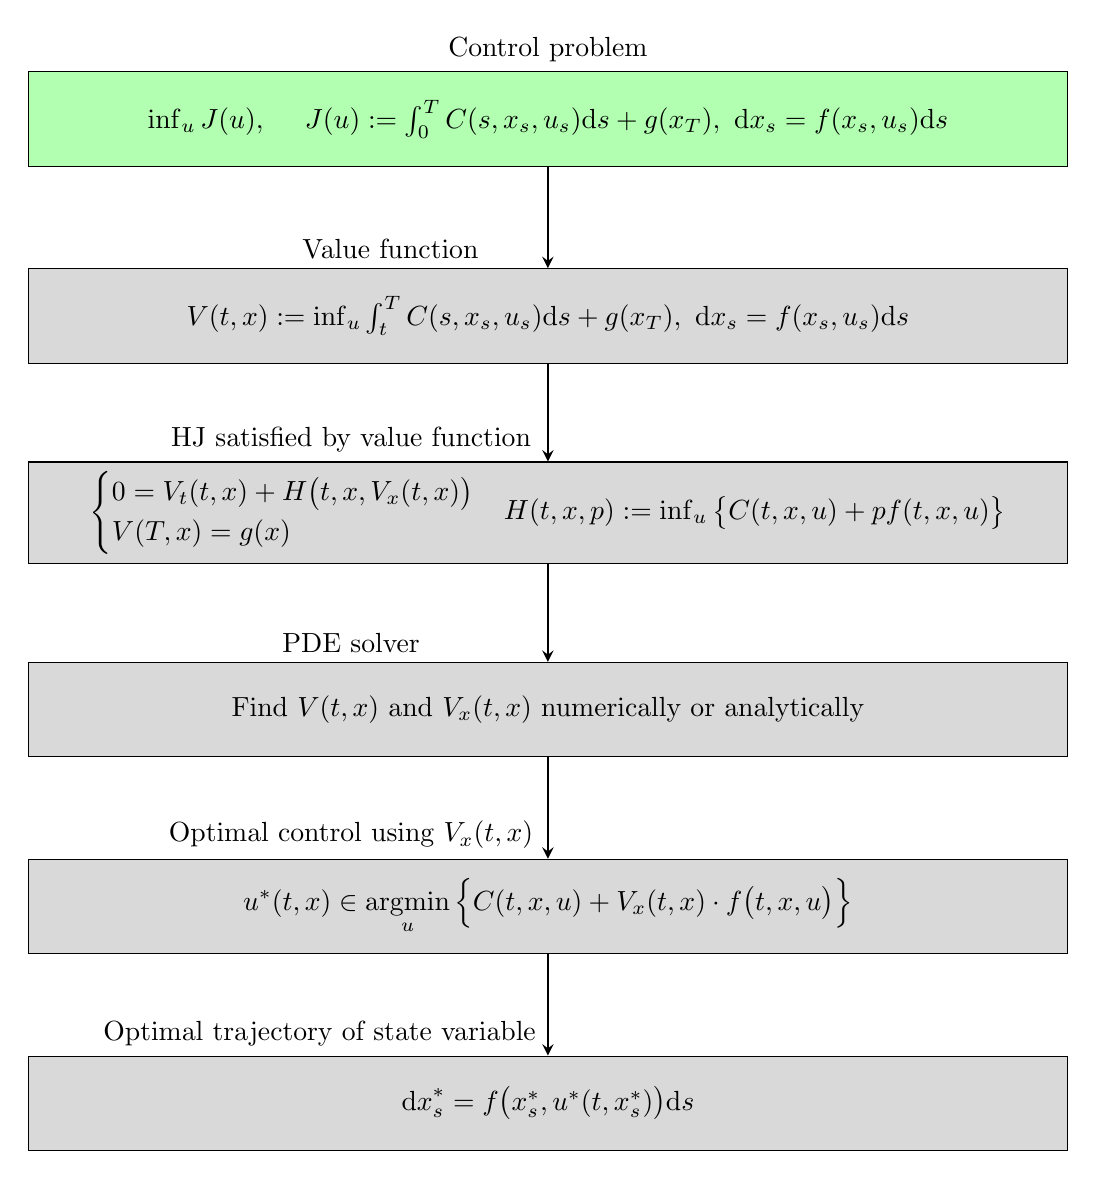
\begin{tikzpicture}[node distance=1.5cm]

% Nodes
\node (control) [box,label={[align=left]Control problem}] {$\inf_{u }J(u),~~~~J(u):=\int_0^T C(s,x_s,u_s){{\ds}}+g(x_T),~{\dx}_s=f(x_s,u_s){{\ds}}$};
\node (value) [nonactivebox, below of=control, yshift=-1cm,label={[align=left,xshift=-2cm]Value function}] {$V(t,x):= \inf_{u}\int_t^TC(s,x_s,u_s){{\ds}}+g(x_T),~{\dx}_s=f(x_s,u_s){{\ds}}$};
\node (hj) [nonactivebox, below of=value, yshift=-1cm,label={[align=left,xshift=-2.5cm]HJ satisfied by value function}] {$
    \begin{cases}
        0=V_t(t,x)+H\big(t,x,V_x(t,x)\big)\\
        V(T,x)=g(x)
    \end{cases}$\\
     $H(t,x,p):=\inf_{u} \big\{C(t,x,u) + pf(t,x,u)\big\}$};
\node (solve) [nonactivebox, below of=hj, yshift=-1cm,label={[align=left,xshift=-2.5cm]PDE solver}]{Find $V(t,x)$ and $V_x(t,x)$ numerically or analytically};    
\node (optimal) [nonactivebox, below of=solve, yshift=-1cm,label={[align=left,xshift=-2.5cm]Optimal control using $V_x(t,x)$}] {$u^*(t,x)\in\mathop{\text{argmin}}\limits_{u}\Big\{C(t,x,u) + V_x(t,x)\cdot f\big(t,x,u\big)\Big\}$};
\node (trajectory) [nonactivebox, below of=optimal, yshift=-1cm,label={[align=left,xshift=-2.9cm]Optimal trajectory of state variable}]{${\dx}^*_s=f\big(x^*_s,u^*(t,x^*_s)\big){{\ds}}$};
\

% Arrows
\draw [arrow] (control) -- (value);
\draw [arrow] (value) -- (hj);
\draw [arrow] (hj) -- (solve);
\draw [arrow] (solve) -- (optimal);
\draw [arrow] (optimal) -- (trajectory);


\end{tikzpicture}

\end{document}
